\documentclass[mathserif]{beamer}

\usetheme{Madrid}

\usepackage{tikz}
\usepackage{url}

\begin{document}

%\begin{frame}{All Classes}[fragile]
%  \begin{Verbatim}[commandchars=\\\{\}]
\PY{k}{use} \PY{n+nn}{MooseX::}\PY{n}{Declare}\PY{p}{;}
\PY{k}{use} \PY{n+nn}{Method::}\PY{n+nn}{Signatures::}\PY{n}{Modifiers}\PY{p}{;}
\end{Verbatim}

%\end{frame}

\begin{frame}{The Challenge: A Flexible Interface to a Complex Model}
  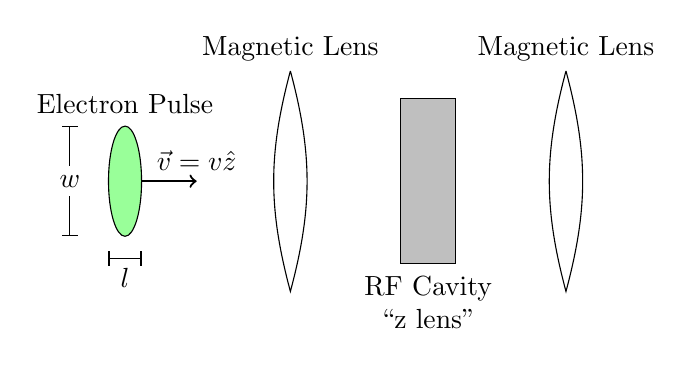
\begin{tikzpicture}[scale=0.7]
    \draw [fill=green!40] (0,0) ellipse [x radius=3mm, y radius=1cm];
    \draw [|-|] (-1,1) -- ++(0,-2) node [pos=0.5,fill=white] {$w$};
    \draw [|-|] (-0.3,-1.4) -- ++(0.6,0) node [pos=0.5,below] {$l$};
    \node at (0, 1.4) {Electron Pulse};
    \draw [thick, ->] (0.3,0) -- ++ (1,0) node [above,pos=1] {$\vec{v} = v \hat{z}$};
    \draw 
      (3,2)
      to [out=-75,in=75] ++(0,-4)
      to [out=105,in=255] ++(0,4)
      node [above] {Magnetic Lens}
    ;
    \draw [fill=gray!50] (5,1.5) rectangle ++(1,-3);
    \node at (5.5,-2.2) [align=center] {RF Cavity\\``z lens''};
    \draw 
      (8,2)
      to [out=-75,in=75] ++(0,-4)
      to [out=105,in=255] ++(0,4)
      node [above] {Magnetic Lens}
    ;
  \end{tikzpicture}
  \begin{itemize}
    \item Compute dynamics of electron pulse
    \item Generation and optical elements add terms to DE
  \end{itemize}
\end{frame}

\begin{frame}{The ``State of the Art''}
  Old codes are
  \begin{itemize}
    \item lacking full 6D dynamics
    \item optimized for performance
    \item hard to customize
    \item near impossible to comprehend
  \end{itemize}
  \begin{block}{\url{http://laacg.lanl.gov/laacg/services/download_sf.phtml}}
    \textbf{Getting Started with Poisson Superfish}\\
    \ldots We do not recommend trying to build an input file ``from scratch.'' Instead, find an example file that is similar to the problem you are trying to solve. Make a copy of the file and then make any necessary modifications to the geometry and options.
  \end{block}
\end{frame}

\begin{frame}{Physical Simulations}
  \begin{block}{Differential Equations}
    A set of rules that define how variables change with some parameter
    \begin{equation*}
      x(t_2) = x(t_1) + \frac{dx}{dt}*dt
    \end{equation*}
  \end{block}
\end{frame}

\begin{frame}{Other Attempts}
  \begin{columns}
    \begin{column}{0.49\linewidth}
      Mathematica:\\
      Pros:
      \begin{itemize}
        \item Can solve dynamics
        \item Pretty-printing of math for readability
      \end{itemize}
      Cons:
      \begin{itemize}
        \item Closed-source and expensive!
        \item No OO and no key-value datatypes
        \item Still rather slow $\sim$2mins$/$sim
      \end{itemize}
    \end{column}
    \begin{column}{0.49\linewidth}
      Modelica:\\
      Pros:
      \begin{itemize}
        \item Open-source, but behind close-source variants
        \item Unique OO language for physical simulation
        \item Classes have DEs as properties
      \end{itemize}
      Cons:
      \begin{itemize}
        \item Lacks ``has-a'' relationship
        \item Composing DEs not trivial
        \item User-facing object instantiation not trivial
        \item Some numerical problems (?)
      \end{itemize}
    \end{column}
  \end{columns}
\end{frame}

\begin{frame}{\ldots But First, Some Bookkeeping}

\end{frame}

\end{document}
